
Ein kurzer Rückblick soll Revue passieren lassen, was wir anfänglich erreichen wollten und wie weit wir gekommen sind. 
\\
\\
Zuerst sollte festgehalten werden, dass wir uns zu Beginn trotz unserer vielen Ideen für ein Basisprodukt entschieden haben, da unsere Erfahrung ausreicht, um einschätzen zu können, dass die Bearbeitungszeit knapp ist, Lieferanten lange Lieferzeiten aufrufen und auch ein Lockdown nicht auszuschließen war. 

\begin{center}
	\textit{Think big, build small!} \cite{Full2022}
\end{center}
Dennoch haben wir den Großteil geschafft, wie im Ausschnitt in Abbildung \ref{trello} unseres aktuellen Trello-Boards  zu erkennen ist.
\begin{figure} [H]
	\begin{center}
		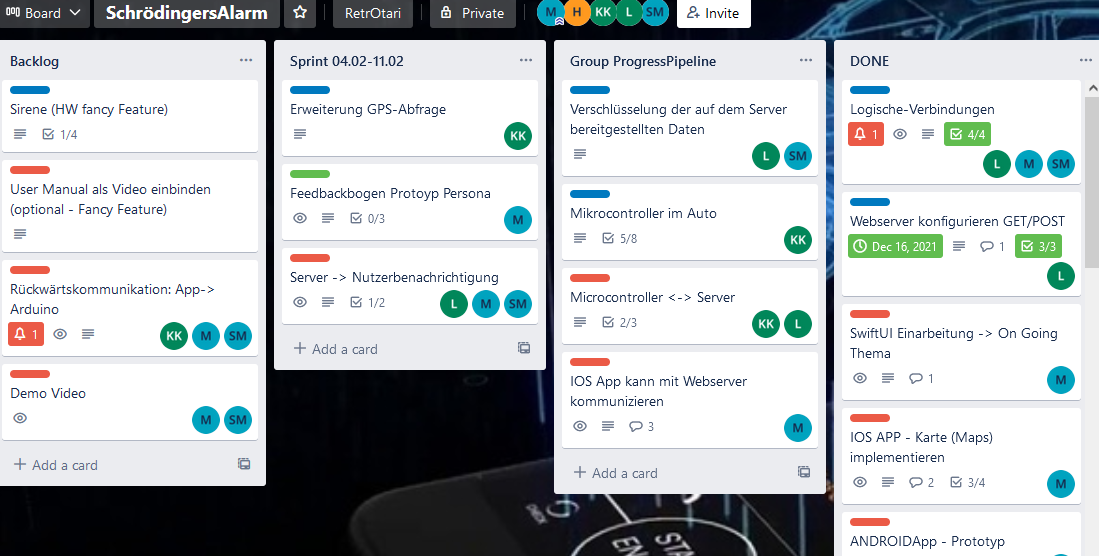
\includegraphics[width=1\textwidth]{Bilder/Rueckblick_Vergleich.png}
		\caption{Abschlussstand Trello-Board}
		\label{trello}
	\end{center}
\end{figure}



\section{Lessons Learned}
Es ist wichtig dass das Minimum Viable Product einen Nutzen bringt und einfach in seiner Bedienung ist\cite{Full2022}
Durch Feedback von unseren Testern konnten wir herauskristallisieren, dass unsere Apps durch ihr derzeitiges unterschiedliches Design irreführend sind - Anmerkung: Ein einheitliches Design an sich war uns bis hier nicht wichtig, da hier tatsächlich der Lernerfolg und Spaß an der Bearbeitung an erster Stelle standen. Dennoch ist dies ein ernstzunehmender Punkt.
\\
\\
Desweiteren wurde sich gewünscht, dass kleine User Manuals für beispielsweise die Systemerweiterung in Form von Kurzvideos bereitgestellt werden - so muss kein Papier verschwendet werden, und bei notwendigen Informations-Updates oder generellen Neuerungen kann dies schnell und einfach digital passieren. Ebenfalls wäre ein Routentracking vorteilhaft, da derzeit immer nur der letzte Standort abgerufen werden kann - so könnte das gestohlene Auto besser nachverfolgt werden. 
\\
\\
Nach so einigen Verbesserungsvorschlägen möchten wir natürlich auch noch festhalten, dass besonders die offene und so leicht erweiterbare Bauweise, die erste ergänzende Idee mit der Sirene, der Geofencing-Mechanismus sowie dass es Apps für beide Betriebssysteme gibt, für sehr positiv empfunden wurden.




\section{Zukünftige Entwicklung}

\textbf{Arduino}
\\
\\
Als Erweiterungen für den Arduino sollen in Zukunft noch eine Alarmsirene vom Typen BSE128 verbaut werden und für die Standorterkennung noch die Google API zur beseren Lokalisierung genutzen werden. 
Für die Sirene muss das Gesamtsystem noch dahingehend erweitert werden, dass eine Kommunikation zum Arduino hin möglich wird. Auf dem Arduino muss hierfür noch realisiert werden, dass der Rückgabewert vom Server abgespeichert wird und in regelmäßigen Abständen geprüft wird, dass sich das Gerät nicht aus dem vom Anwender definierten Bereich entfernt hat. Es muss also noch Geofencing ermöglicht werden, um zu erkennen wann die Sirene auslösen soll. Es ist aber auch eine einfache Lösung denkbar, bei der der Benutzer den Alarm aus der Entfernung selbst steuern muss bzw kann.
\\
Aus Hardware Sicht muss dann nur die Sirene mittels Transistorschaltung an den Arduino angeschlossen und mit Strom versorgt werden, damit der Arduino das Alarmsignal im Fall einer Entwendung geben kann. Die Schaltung dafür sieht wie folgt aus:
\begin{figure} [H]
	\begin{center}
		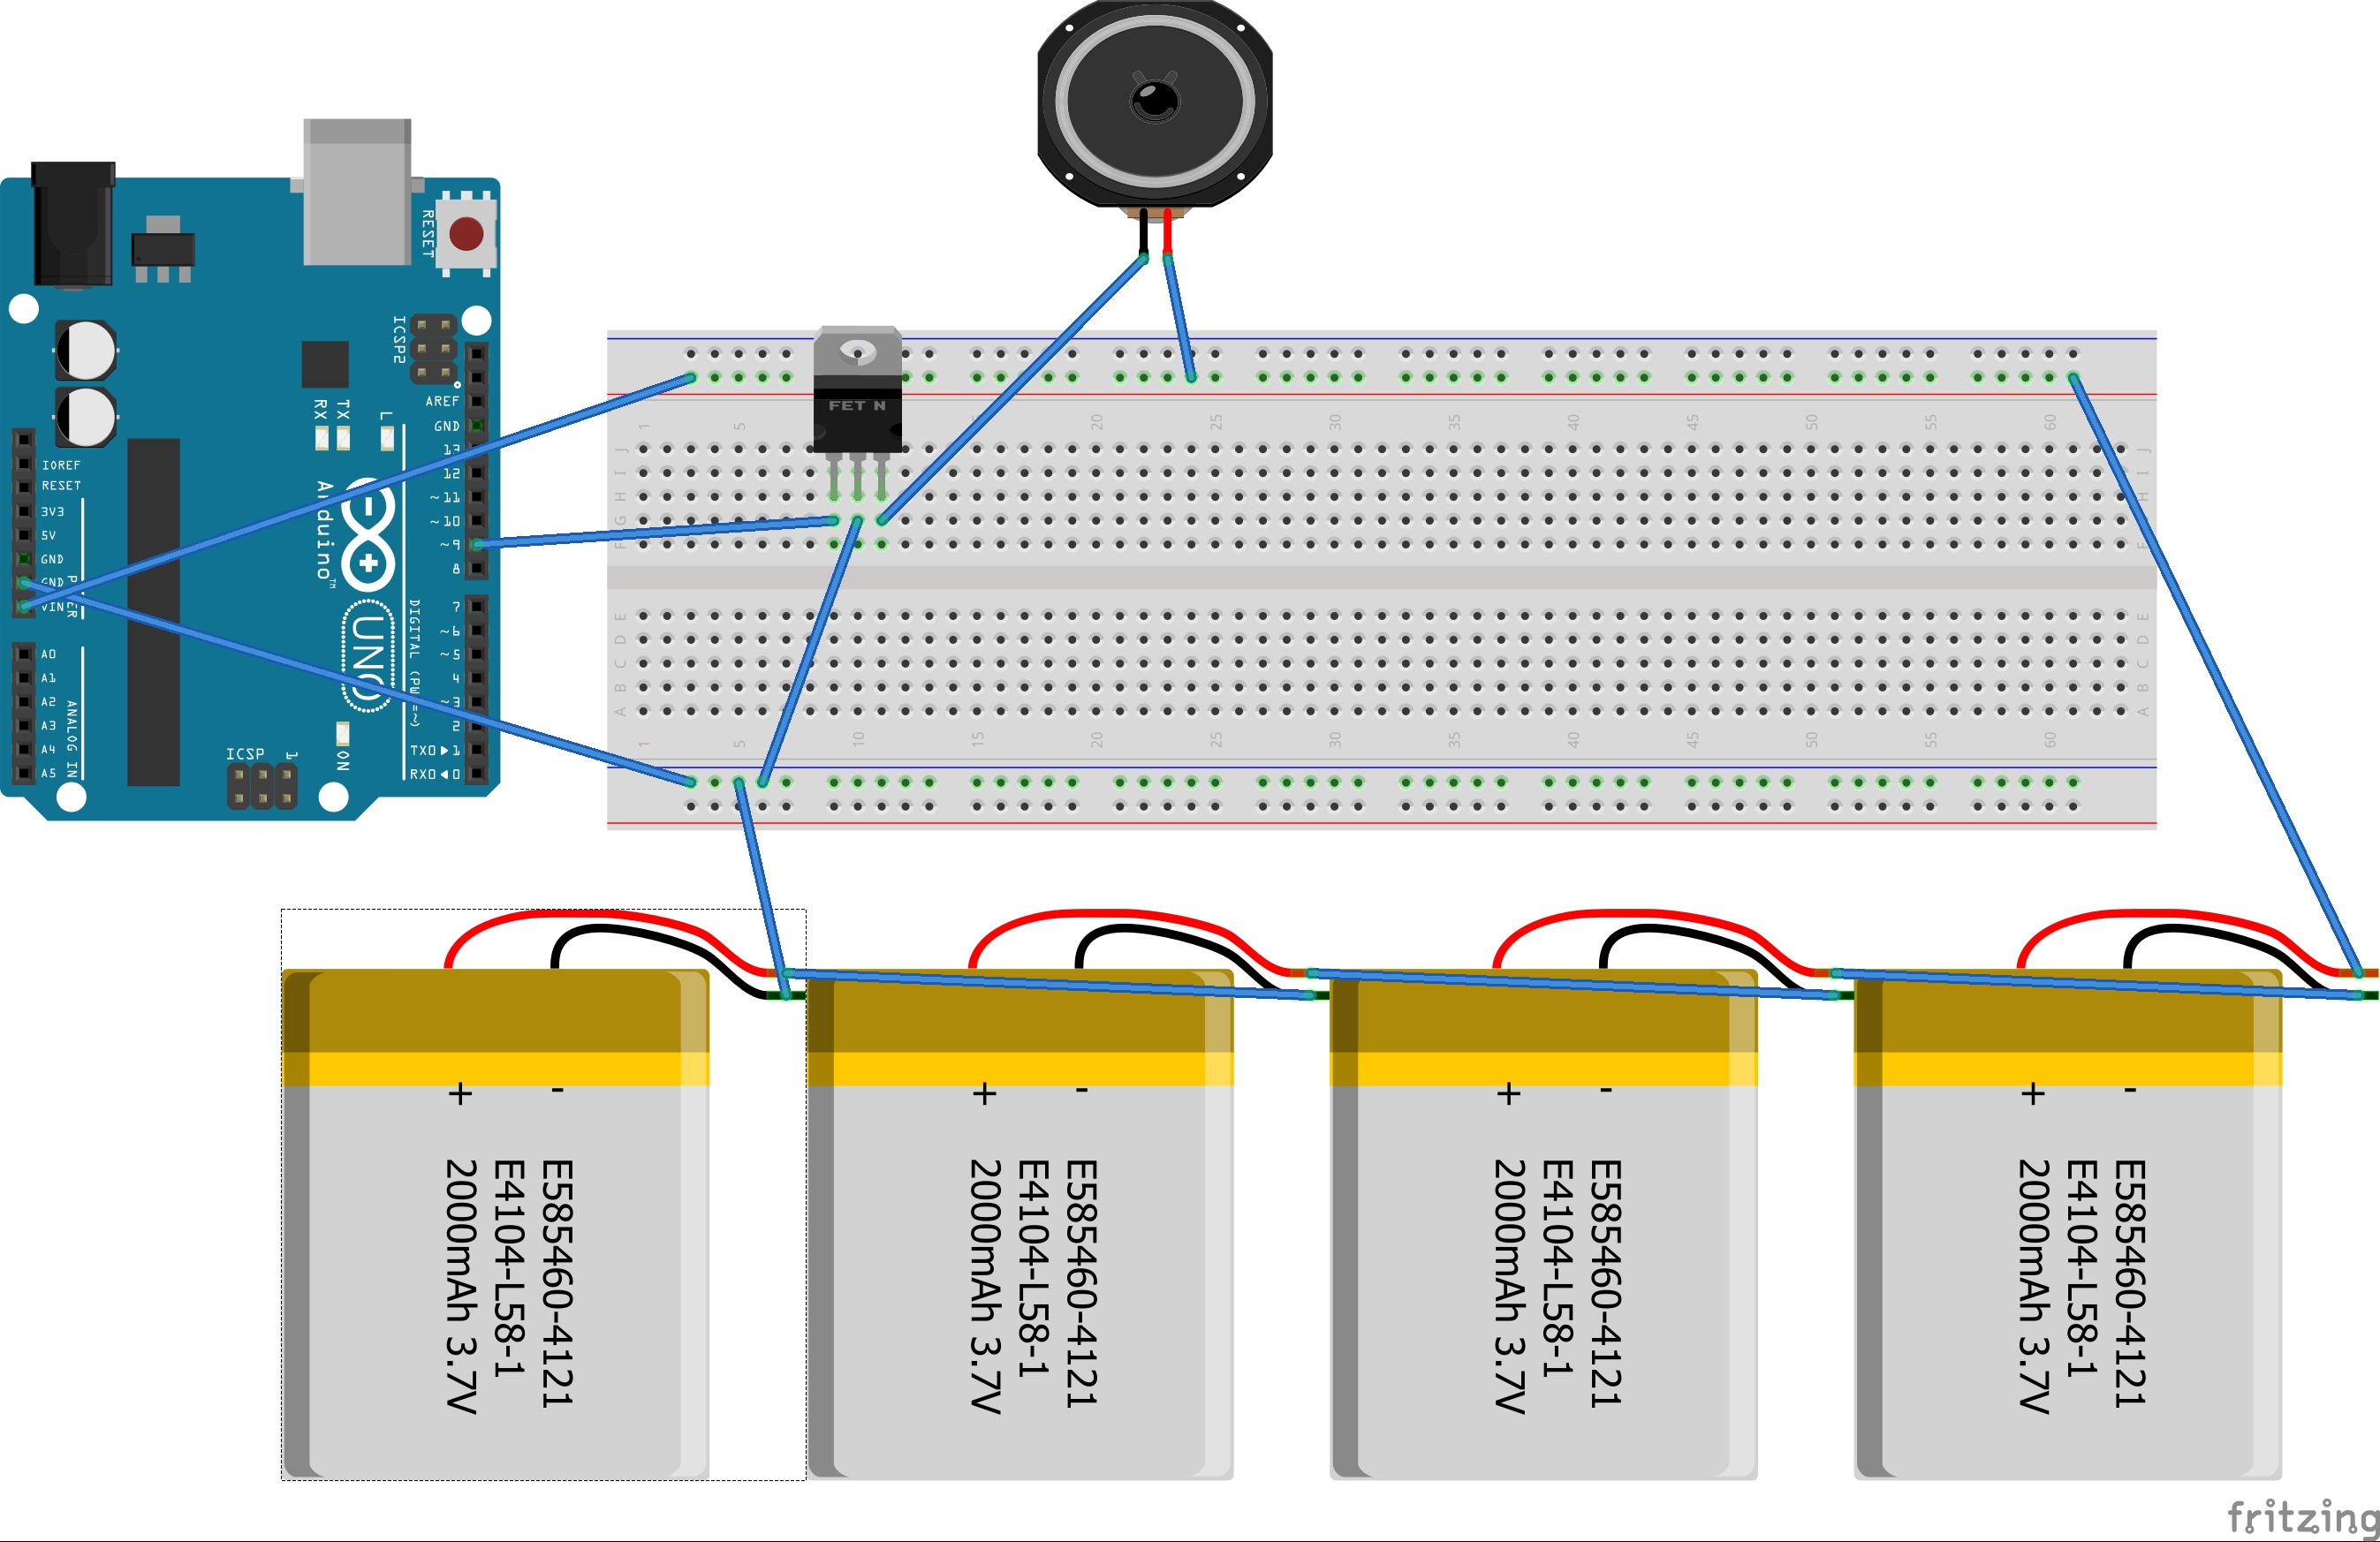
\includegraphics[width=1\textwidth]{Bilder/Arduino_Sirene.jpg}
		\caption{Systemerweiterung um Sirene}
		\label{sirene}
	\end{center}
\end{figure}
Dabei kann die Sirene, da sie 12-24V Eingangsspannung akzeptiert, an die Stromversorgung des Arduinos mit angeschlossen werden. Es muss dafür jedoch eventuell die Akkuleistung ebenfalls erweitert werden. Dies muss jedoch erst noch getestet werden. 
\\
\\
Die Sirene soll zukünftig durch eine einfache N-Channel Mosfet Schaltung gesteuert werden.
Um den Google Standort Service effektiv verwenden zu können, ist die Erweiterung um einen WLAN Empfänger sinnvoll. Somit kann neben den Informationen, die durch GSM und GPS zur Verfügung stehen, auch die lokalen WLAN-Netze zur Standortermittlung genutzt werden. Dies erhöht weiter die Genauigkeit kann aber theoretisch auch wegfallen. Die Verwendung der API ist jedoch kostenpflichtig und dementsprechend ist das Geschäftskonzept eventuell weiter zu überdenken. Eine mögliche Lösung hierfür wäre ein monatliches Bezahlkonzept, über das man je nach Bedarf die API Standorterkennung hinzu buchen kann.
\\
\\
\textbf{Webserver} 
\\
\\
\textit{Finalisierung der Verschlüsselung}
Der erste Punkt, der in Zukunft bearbeitet werden soll, ist die vollständige Implementierung und ein anschließendes Testen der Verschlüsselung der Nutzdaten. Für den Webserver ist wie zuvor beschrieben bereits alles fertig. Es gilt nun also die entsprechend umgekehrten Abläufe in den beiden Apps zu realisieren.
\\
\\
Darüber hinaus sollte geprüft werden, ob es auch möglich ist, die Koordinaten bereits auf dem Arduino zu verschlüsseln. So könnte zusätzliche Sicherheit der Daten gewonnen werden.
\\
\\
\textit{Umstellung auf HTTPS}
\\
Bei der Entwicklung der iOS-App trat an der Stelle des Auslesens der JSON codierten Daten ein Problem auf. Die Fehlermeldungen waren zunächst nicht eindeutig zu interpretieren, doch es stellte sich heraus, dass mit der von uns gewählten Version nur von HTTPS-Seiten JSONs mittels HTTP-GET abgefragt werden können.
\\
\\
Um derartige Probleme in Zukunft zu umgehen, soll der Webserver von HTTP auf HTTPS umgestellt werden. Wir hatten auch erst überlegt, dies im aktuellen Bearbeitungszeitraum umzusetzen, jedoch fand sich für die iOS-App eine Alternativlösung. Auch erste Recherchen zur Umstellung auf HTTPS zeigten uns, dass dies doch ziemlich aufwendig werden und wieder neue Probleme mit sich bringen könnte.
\\
\\
\textit{Bidirektionale Kommunikation ermöglichen}
\\
Ein weiteres Feature, das in Zukunft realisiert werden soll, ist eine Kommunikation auch in die andere Richtung. Es soll also dann möglich sein, dass die App Befehle oder sonstige Daten an den Webserver schickt und der Arduino diese dann auch abfragen kann. Eine solche Kommunikation wäre zum Beispiel für das Aktivieren der ebenfalls noch geplanten Sirene im Innenraum des Fahrzeugs erforderlich.
\\
\\
\textit{MQTT als redundanten Übertragungsweg einrichten}
\\
Um nicht nur den bisherigen Übertragungsweg über den HTTP-Server nutzen zu können und somit anfällig für Systemausfälle zu sein, soll ein zweiter, redundanter Übertragungsweg mit Hilfe des MQTT-Protokolls errichtet werden. Hierfür ist als erstes das Bereitstellen eines eigenen MQTT-Brokers erforderlich, um direkt unabhängig von Dritten zu sein. Auch muss ein MQTT-Topic definiert werden, in welchem die Kommunikation stattfinden soll. Im nächsten Schritt muss auf dem Arduino ein entsprechendes Skript programmiert werden, mit welchem die Koordinaten mittels PUBLISH zum MQTT-Broker übermittelt werden können. Dieses muss dann entweder parallel zum bisherigen Skript ausgeführt werden oder es werden beide in einem neuen Skript vereinigt.
\\
\\
Anschließend muss in den beiden Apps ein MQTT-SUBSCRIBE implementiert werden, um die vom Arduino veröffentlichten Daten zu erhalten. Auch dies muss parallel zur Datenabfrage vom Webserver geschehen. Zusätzlich soll in den Apps dann ein Abgleich beider Daten (HTTP und MQTT) implementiert werden. Sind beide Daten gleich werden die neuen Koordinaten übernommen. Für den anderen Fall, dass die beiden Datenpakete unterschiedlich sind, muss noch überprüft werden, welche Daten dann gespeichert werden. 
\\
\\
\textbf{Apps} 
\\
\\
\textit{Datenbanken}
\\
Für spätere Versionen sollten  Möglichkeiten einer Datenbank-Einbindung beispielsweise mit "Firebase", um die Datenbankverwaltung besser zu verwalten, implementiert werden. 
\\
\\
\textit{Routentracker}
\\
Die Idee ist nicht neu und dennoch sehr praktisch - damit nicht nur der aktuelle Standort angezeigt wird, sondern auch eine Nachverfolgung, wäre eine Art Routentracker sinnvoll. Dafür müssten in der JSON-Datei mehrere Daten in einem zuvor definierten Intervall abgespeichert werden, welche dann als verbundene Punkte auf der Karte angezeigt werden. So kann im Falle eines Diebstahl die ganze Strecke nachvollzogen werden, die bereits zurückgelegt wurde.
\\
\\
\textit{Android- \& Apple-Watch Kommunikation}
\\
Smartwatches liegen im Trend und Smartphones werden immer größer und dadurch schnell unhandlich, so dass sie gerne in einer Tasche verstaut werden. Daher ist es eine nützliche Überlegung, dass die Apps auch für Smartwatches bereitgestellt werden, so dass der Nutzer noch schneller bemerkt, wenn ein Alarm ausgelöst wird.
\\
\\
\textit{Eine App - Mehrere Fahrzeuge}
\\
Es ist sinnvoll, dass wenn man von mehreren Alarmsystemen in Fahrzeugen ausgeht, dass die App gesagt bekommt, welches Gerät der Nutzer Zuhause besitzt - daher sollte es eine Konfigurationsmöglichkeit innerhalb der App für das Alarmsystemgerät geben. Des weiteren wäre es auch sinnvoll, dass wenn beispielsweise eine Familie mit mehreren Systemen und unterschiedlichen Fahrzeugen diese sich in der App  gebündelt anzeigen lassen könnte - da wir derzeit jedoch nur ein System besitzen, wurde es hier erst einmal als Placeholder implementiert.
\begin{figure} [H]
	\begin{center}
		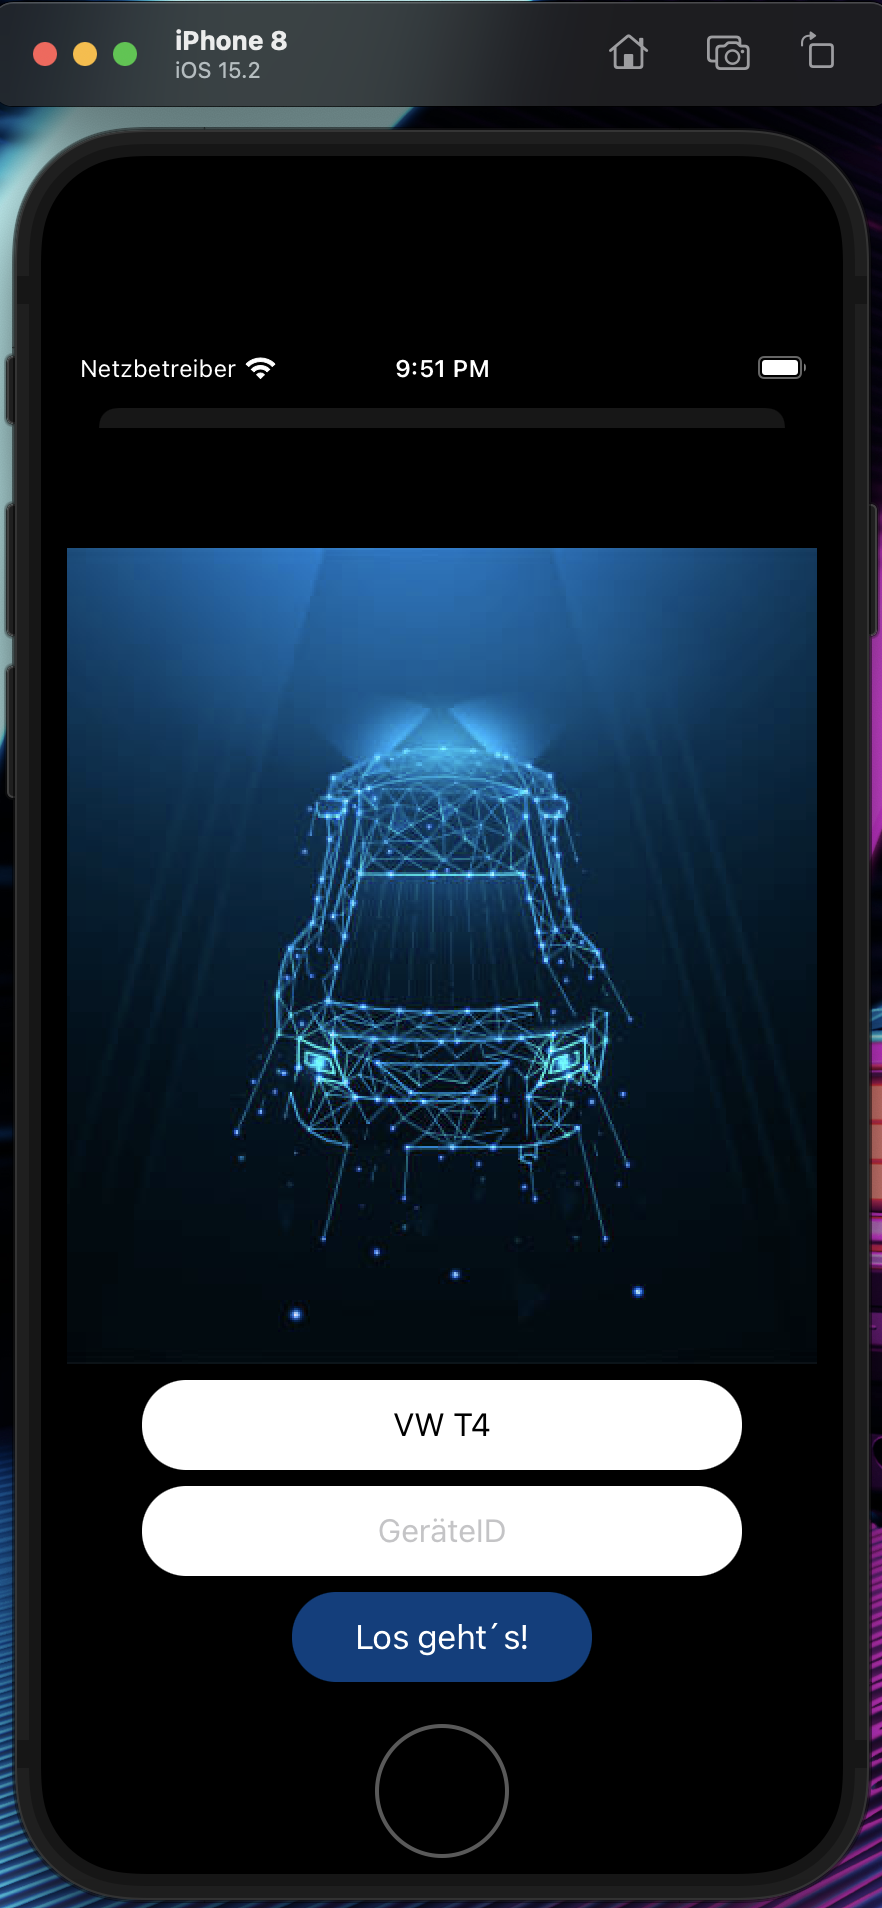
\includegraphics[width=1\textwidth]{Bilder/iOS_addDevice.png}
		\caption{Navigationstab \textit{Fahrzeug hinzufügen}}
		\label{add}
	\end{center}
\end{figure}

\section{Fazit}
Das Projekt war eine wertvolle Erfahrung in vielen Hinsichten - so haben wir nicht nur aus dem Studium bekannte, sondern auch neue Technologien kennengelernt und erprobt. Des weiteren haben wir erfahren, was es bedeutet, ein Produkt von einer kleinen Idee bis hin zu einem umfangreichen funktionierenden Prototypen zu gestalten, entwerfen und aufzubauen. Das Projekt wird uns sicherlich mit all seinen Facetten noch lange im Gedächtnis bleiben und der ein oder andere wird es sicherlich noch weiterentwickeln.